%%
%% This is file `sample-sigplan.tex',
%% generated with the docstrip utility.
%%
%% The original source files were:
%%
%% samples.dtx  (with options: `sigplan')
%% 
%% IMPORTANT NOTICE:
%% 
%% For the copyright see the source file.
%% 
%% Any modified versions of this file must be renamed
%% with new filenames distinct from sample-sigplan.tex.
%% 
%% For distribution of the original source see the terms
%% for copying and modification in the file samples.dtx.
%% 
%% This generated file may be distributed as long as the
%% original source files, as listed above, are part of the
%% same distribution. (The sources need not necessarily be
%% in the same archive or directory.)
%%
%% The first command in your LaTeX source must be the \documentclass command.
\documentclass[sigplan,anonymous,review]{acmart}

%%
%% \BibTeX command to typeset BibTeX logo in the docs
\AtBeginDocument{%
  \providecommand\BibTeX{{%
    \normalfont B\kern-0.5em{\scshape i\kern-0.25em b}\kern-0.8em\TeX}}}

%% Rights management information.  This information is sent to you
%% when you complete the rights form.  These commands have SAMPLE
%% values in them; it is your responsibility as an author to replace
%% the commands and values with those provided to you when you
%% complete the rights form.
\setcopyright{acmcopyright}
\copyrightyear{2019}
\acmYear{2019}
%\acmDOI{10.1145/1122445.1122456}

%% These commands are for a PROCEEDINGS abstract or paper.
\acmConference[GPCE `19]{GPCE '19: 18th International Conference on Generative Programming: Concepts \& Experiences}{October 21--22, 2019}{Athens, Greece}
\acmBooktitle{GPCE `19: 18th International Conference on Generative Programming: Concepts \& Experiences , October 21--22, 2019, Athens, Greece}
\acmPrice{}
\acmISBN{}


%%
%% Submission ID.
%% Use this when submitting an article to a sponsored event. You'll
%% receive a unique submission ID from the organizers
%% of the event, and this ID should be used as the parameter to this command.
%\acmSubmissionID{3}

%%
%% The majority of ACM publications use numbered citations and
%% references.  The command \citestyle{authoryear} switches to the
%% "author year" style.
%%
%% If you are preparing content for an event
%% sponsored by ACM SIGGRAPH, you must use the "author year" style of
%% citations and references.
%% Uncommenting
%% the next command will enable that style.
%%\citestyle{acmauthoryear}

% Packages
\usepackage[inline]{enumitem}
\usepackage[tdiagram]{semantic}
\usepackage{tikz}
\usetikzlibrary{matrix,backgrounds,arrows,decorations.markings}
\tikzset{
  big arrow/.style={
    decoration={markings,mark=at position 1 with {\arrow[scale=2,#1]{>}}},
    postaction={decorate},
    shorten >=0.4pt,
    dashed=true},
  big arrow/.default=red,
}
\usepackage{subcaption} % subfigure
\usepackage{relsize} % large maths symbols

% Commands
\newcommand{\AMcomment}[1]{\textcolor{blue}{[\textbf{AM:} #1]}}
\newcommand{\mslang}{$\lambda_{\uparrow\downarrow}$}
\newcommand{\mslangStar}{$\lambda_{\uparrow\downarrow}^*$}
\newcommand{\mevl}{$M_{e}$}
\newcommand{\secdlisp}{SecdLisp}
\newcommand{\ts}{\textquotesingle}

\theoremstyle{definition}
\newtheorem{definition}{Definition}[section]
\newtheorem{observation}{Observation}[section]

\newcommand{\note}[1]{{\color{red}[#1]}}
\newcommand{\todo}[1]{\note{TODO: #1}}
%\newcommand{\todo}[1]{}

%%
%% end of the preamble, start of the body of the document source.
\begin{document}

%%
%% The "title" command has an optional parameter,
%% allowing the author to define a "short title" to be used in page headers.
\title{Collapsing Heterogeneous Towers of Interpreters}
%Or Collapsing Heterogeneous Towers of Evaluators?

%%
%% The "author" command and its associated commands are used to define
%% the authors and their affiliations.
%% Of note is the shared affiliation of the first two authors, and the
%% "authornote" and "authornotemark" commands
%% used to denote shared contribution to the research.
\author{Michael Buch}
%\authornote{Both authors contributed equally to this research.}
\affiliation{\institution{University of Cambridge}}
\email{mb2244@cam.ac.uk}

\author{Nada Amin}
%\authornotemark[1]
\affiliation{\institution{University of Cambridge}}
\email{na482@cl.cam.ac.uk}

\author{Alan Mycroft}
\affiliation{\institution{University of Cambridge}}
\email{Alan.Mycroft@cl.cam.ac.uk}

%%
%% By default, the full list of authors will be used in the page
%% headers. Often, this list is too long, and will overlap
%% other information printed in the page headers. This command allows
%% the author to define a more concise list
%% of authors' names for this purpose.
\renewcommand{\shortauthors}{Buch, Amin and Mycroft}

%%
%% The abstract is a short summary of the work to be presented in the
%% article.
\begin{abstract}
A tower of interpreters is a program architecture consisting of a sequence of interpreters each interpreting the one above it. The overhead of multiple layers of interpretation can be optimized away using partial evaluation, a process referred to as \textit{collapsing towers of interpreters}.
Previous work has focused on homogeneous towers and their reflective and meta-circular aspects. We explore collapsing \textit{heterogeneous} towers of interpreters, particularly addressing the issues caused by their varying data representations.
\end{abstract}

%%
%% The code below is generated by the tool at http://dl.acm.org/ccs.cfm.
%% Please copy and paste the code instead of the example below.
%%
\begin{CCSXML}
<ccs2012>
<concept>
<concept_id>10011007.10011006.10011041.10010943</concept_id>
<concept_desc>Software and its engineering~Interpreters</concept_desc>
<concept_significance>500</concept_significance>
</concept>
<concept>
<concept_id>10011007.10011006.10011041.10011047</concept_id>
<concept_desc>Software and its engineering~Source code generation</concept_desc>
<concept_significance>500</concept_significance>
</concept>
<concept>
<concept_id>10011007.10011006.10011039.10011311</concept_id>
<concept_desc>Software and its engineering~Semantics</concept_desc>
<concept_significance>100</concept_significance>
</concept>
<concept>
<concept_id>10011007.10011006.10011041.10011046</concept_id>
<concept_desc>Software and its engineering~Translator writing systems and compiler generators</concept_desc>
<concept_significance>100</concept_significance>
</concept>
</ccs2012>
\end{CCSXML}

\ccsdesc[500]{Software and its engineering~Interpreters}
\ccsdesc[500]{Software and its engineering~Source code generation}
\ccsdesc[100]{Software and its engineering~Semantics}
\ccsdesc[100]{Software and its engineering~Translator writing systems and compiler generators}

%%
%% Keywords. The author(s) should pick words that accurately describe
%% the work being presented. Separate the keywords with commas.
\keywords{interpreters, partial evaluation, metaprogramming}

%% A "teaser" image appears between the author and affiliation
%% information and the body of the document, and typically spans the
%% page.
%\begin{teaserfigure}
%  \includegraphics[width=\textwidth]{sampleteaser}
%\end{teaserfigure}

%%
%% This command processes the author and affiliation and title
%% information and builds the first part of the formatted document.
\maketitle

\section{Introduction}
Towers of interpreters are a program architecture which consists of sequences of interpreters where each interpreter is interpreted by an interpreter above it (depicted as a tombstone diagram in figure \ref{fig:tombstone_tower_ex1}). Each additional \textit{level} (i.e., interpreter) in the tower adds a constant factor of interpretative overhead to the run-time of the system. One of the earliest mentions of such architectures in literature is a language extension to Lisp called 3-LISP~\cite{smith1984reflection} introduced by Smith. Smith describes the notion of a reflective system, for ``a system that is able to reason
about itself'', as a tower of meta-circular interpreters, also referred to as a \textit{reflective tower}\footnote{
Reflective towers are often theorised as infinite, but any finite
computation only uses a bounded number of layers.}.
% in theory are  are considered to be potentially infinite. Given enough computing resources one can create towers consisting of an unbounded number of interpreters.}.
Using this architecture 3-LISP enables an interpreter within the tower to access and modify internal state of its neighbouring interpreters. An interpreter is \textit{meta-circular} when the language the interpreter is written in and the language it is interpreting are the same. Meta-circularity and the common data representation between interpreters are core properties of reflective towers studied in previous work. We refer to towers with such properties as \textit{homogeneous}.

\begin{figure}[t]
    \centering
        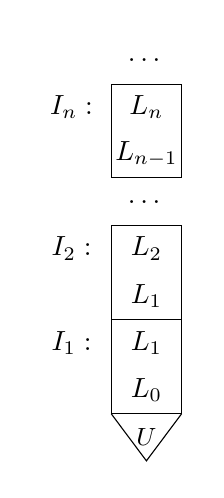
\begin{tikzpicture}
            \matrix (m) [matrix of nodes,nodes={minimum width=2.5em,minimum  height=1.7em}
                        ]
            {
                         & \dots                   \\
                $I_n:$   & $L_n$                   \\
                         & $L_{n-1}$               \\
                         & \dots                   \\
                $I_2:$   & $L_2$                   \\
                         & $L_1$                   \\
                $I_1:$   & $L_1$                   \\
                         & $L_0$                   \\
                         & |[font=\small]|$U$      \\
              };
              \draw (m-1-2.south west) |- (m-4-2.north east) |- (m-1-2.south west);
              \draw (m-4-2.south west) |- (m-6-2.south east) |- (m-4-2.south west);
              \draw (m-4-2.south west) |- (m-8-2.south east) |- (m-6-2.north east);
              \draw (m-8-2.south west) -- (m-9-2.south) -- (m-8-2.south east);
        \end{tikzpicture}
    \caption{A tower of interpreters where each interpreter $I_n$ is written in language $L_{n-1}$ and interprets a language $L_n$, for some $n \geq 0$. In literature the tower often grows downwards, however, in our study we refer to $I_0$ as the base interpreter and grow the tower upwards for convenience. $U$ is the underlying machine (e.g. CPU) on which the base interpreter is executed.}
    \label{fig:tombstone_tower_ex1}
\end{figure}

In the original reflective tower models only minimal attention was given to the cost of performing new interpretation at each level of a tower. Then works by Sturdy~\cite{sturdy1993lisp} and Danvy et al.'s language Blond~\cite{danvy1988intensions} hinted at the possibility of removing some of this overhead by partially evaluating (i.e., specializing) interpreters with respect to the interpreters below in the tower. Asai et al.'s language Black~\cite{asai1996duplication} is a reflective language implemented through a reflective tower. The authors use a hand-crafted partial evaluator, and in a later study use MetaOCaml~\cite{asai2015compiling}, to efficiently implement the language. Asai and then, using the language Pink~\cite{amin2017collapsing}, Amin et al.~demonstrate the ability to compile a reflective language even though the semantics of individual interpreters in the underlying tower can be modified. Essentially this is achieved by specializing and executing functions of an interpreter at run-time to remove the cost of multiple interpretation; this effectively \textbf{\textit{collapses}} a tower.

Parallel to all the above theoretical research into reflective towers, practical programmers have in effect been working with towers of interpreters dating back to the idea of language parsers. Writing a parser in an interpreted language already implies two levels of interpretation:
one running the parser and another the parser itself. Emulation is a form of interpretation and implies interpreters running on virtual hardware, such as the bytecode interpreter in the Java Virtual Machine (JVM)~\cite{lindholm2014java}, are towers of interpreters as well.

However, these two branches of research do not overlap and work on towers of interpreters rarely studied their counterparts in production systems. It is natural to ask the question of what it would take to apply previous techniques in partial evaluation to a practical setting. This is the question Amin et al. pose in their conclusion after describing Pink~\cite{amin2017collapsing} and is the starting point for this work.

We aim to bring previous work of removing interpretative overhead in towers using partial evaluation into practice. Our study achieves this by constructing a proof-of-concept tower of interpreters that more-closely resembles those in real-world systems. Figure \ref{fig:tombstone} depicts two versions of our experimental tower. Traditionally reflective towers are thought of as completely vertical like the one on the left. However, details such as how a tower grows, shrinks and collapses while executing user programs worked rather mysteriously. We decided to implement our tower using occasional layers of compilation (as shown on the right). The two versions of our tower are extensionally equal since they yield the same output for a given program to evaluate. Part of our study is devoted to evaluating the effect of the intensional structure of towers on the act of collapsing them.

We then collapse the experimental tower under different configurations and evaluate the resulting optimized programs. We demonstrate that we can partially evaluate individual interpreters in a heterogeneous tower and effectively generate code specialized for a user program (hopefully eliminating interpretative overhead in the process).
Our contributions include:
\begin{enumerate}
\item Develop an experimental heterogeneous tower of interpreters, with a SECD machine~\cite{landin1964mechanical,kogge1990architecture} in between two Lisp-like levels
\item Collapse this heterogeneous tower, removing all interpretation overhead
\item Identify general requirements and strategies for collapsing heterogeneous towers
\end{enumerate}

In
section~\ref{subsec:collapse}, we describe what it means to construct
and collapse a tower of interpreters and the methodology Pink
uses to do so~\cite{amin2017collapsing}. In
section~\ref{sec:heterogeneity}, we discuss heterogeneous towers
and in section~\ref{subsec:collapseh}, how to collapse them.
In section~\ref{sec:conc}, we conclude, looking back and ahead.
Our experiments are available from \textit{**omitted for double-blind review**}.

\begin{figure*}
    \centering
    \hspace*{1.5cm}
    \begin{subfigure}{0.3\linewidth}
    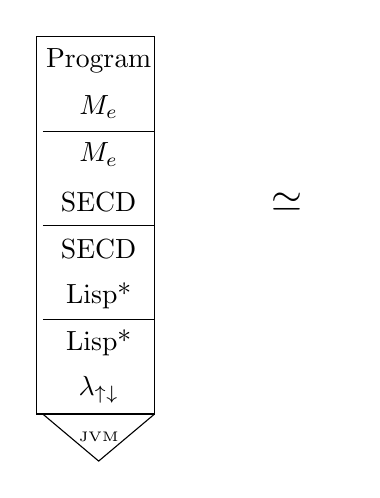
\begin{tikzpicture}
        \matrix (m) [matrix of nodes,nodes={minimum width=4em,minimum  height=1.7em}]
        {
            Program                 \\
            \mevl                   \\
            \mevl                   \\
            SECD &[6ex] $\boldsymbol{\mathlarger{\mathlarger{\mathlarger{\simeq}}}}$   \\
            SECD                    \\
            Lisp*                   \\
            Lisp*                   \\
            \mslang                 \\
            |[font=\tiny]|JVM       \\
          };
          
          %Without arc
          \draw (m-1-1.north west) |- (m-8-1.south east) |- (m-1-1.north west);

          \draw (m-2-1.south west) -- (m-2-1.south east);
          \draw (m-4-1.south west) -- (m-4-1.south east);
          \draw (m-6-1.south west) -- (m-6-1.south east);
          \draw (m-8-1.south west) -- (m-9-1.south) -- (m-8-1.south east);
    \end{tikzpicture}
    \end{subfigure}
    \begin{subfigure}{0.6\linewidth}
    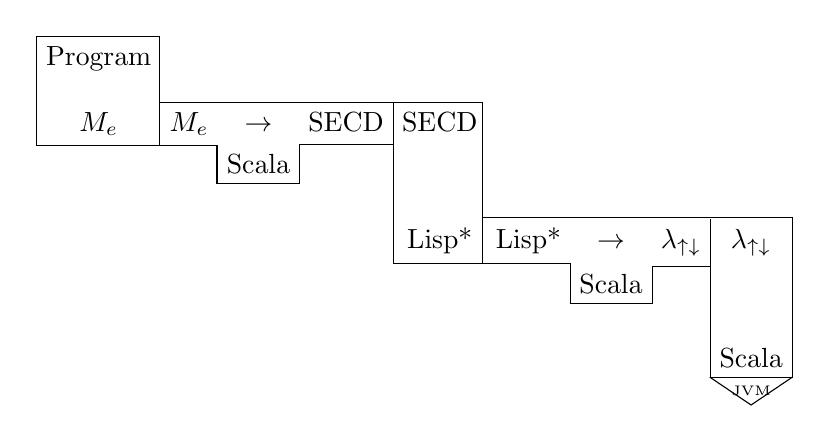
\begin{tikzpicture}
    \matrix (m) [matrix of nodes]
    {
     Program   &        &       &        &      &                                               \\[2ex]
       \mevl   &  \mevl &  $\to$ &  SECD & SECD &                                               \\
               &        &  Scala &                                                              \\[3ex]
               &        &    &       & Lisp* & Lisp* & $\to$ & \mslang & \mslang                \\
               &        &    &       &      &        & Scala &                                  \\[3ex]
               &        &    &       &      &        &       &         &  Scala                 \\
               &        &    &       &      &        &       &         &  |[font=\tiny]|JVM     \\
      };

    %Without arc
    \draw (m-1-1.north west) |- (m-2-2.south west) |- (m-1-1.north west);

    \draw (m-2-2.south west) |- (m-2-4.north east) |- (m-3-3.north east) |- (m-3-3.south west) |- (m-2-2.south west);
    \draw (m-2-4.north east) |- (m-4-5.south east) |- (m-2-4.north east);
    \draw (m-4-5.south east) -- (m-4-6.south east) |- (m-5-7.south east) |- (m-4-8.south east) |- (m-6-9.south east)
            |- (m-4-5.north east);
    \draw (m-4-8.north east) -- (m-4-8.south east);
    \draw (m-6-9.south west) -- (m-7-9.south) -- (m-6-9.south east);
    \end{tikzpicture}
    \end{subfigure}
    \caption{Tombstone diagrams that represent two versions of our experimental tower of interpreters. \mevl{} is a toy Lisp language, \mslang{} refers to the multi-level language introduced as part of Pink~\cite{amin2017collapsing} and Lisp* is \mslang's Lisp based front-end. \textit{JVM} in our diagram also encompasses any underlying machinery necessary to run it. While the left depicts the intuitive view of a tower, we actually implement it using the architecture on the right. Not only is the tower on the right simpler to construct but it also highlights the power of the \textit{lift} operator and its vital role in collapsing heterogeneous towers.
}
    \label{fig:tombstone}
\end{figure*}

%\section{Background}\label{sec:background}
%\subsection{SECD}\label{subsec:secd}
%\subsection{Partial Evaluation}\label{subsec:pe}
\section{Collapsing Reflective Towers}\label{subsec:collapse}

\textit{Collapsing} a tower means removing overhead from multiple interpretation. To do so we specialize our tower with respect to a user program and produce a residual program with as little interpretation left as possible. The three key ingredients for collapsing a tower using Pink's technique~\cite{amin2017collapsing} are:
\begin{enumerate}
    \item A multi-level language
    \item A \textit{lift} operator
    \item A \textit{stage-polymorphic} evaluator
\end{enumerate}
Amin et al.'s multi-level language, \mslang, differentiates between static and dynamic (i.e., code) expressions using constructors;
this allows \mslang{} to express binding-time information. The
\textit{lift} operator coerces static to dynamic values, in the style
of the reification operator of Type-Directed Partial Evaluation (TDPE)~\cite{danvy1999type}.
To stage the evaluator, the usual recipe applies: introductory forms that
produce values are lifted, while elimination forms that consume values
remain unchanged (the result will be dynamic if the operands are
dynamic, and static if the operands are static). An evaluator can be
made \textit{stage-polymorphic}, parameterized over whether to be
staged (acting as a compiler) or not (acting as an interpreter) by
taking as argument a \textit{maybe-lift} function that acts as the
\textit{lift} operator or the identity function, respectively.

\begin{figure}
    \centering
    \begin{subfigure}{.4\linewidth}
    \centering
        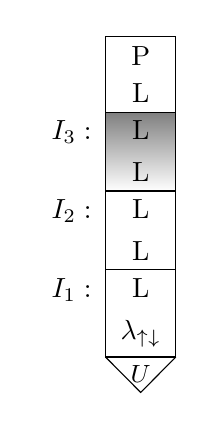
\begin{tikzpicture}
            \matrix (m) [matrix of nodes,nodes={minimum width=2.5em,minimum  height=1.2em}
                        ]
            {
                            &   P                           \\
                            &   L                           \\
             $I_3:$         &   L                           \\
                            &   L                           \\
             $I_2:$         &   L                           \\
                            &   L                           \\
             $I_1:$         &   L                           \\
                            &   \mslang                     \\
                            &   |[font=\small]|$U$          \\
              };
            \draw (m-1-2.north west) |- (m-8-2.south east) |- (m-1-2.north west);
            \draw (m-2-2.south west) -- (m-2-2.south east);
            \draw (m-4-2.south west) -- (m-4-2.south east);
            \draw (m-6-2.south west) -- (m-6-2.south east);
            \draw (m-8-2.south west) -- (m-9-2.south) -- (m-8-2.south east);

            % Background
            \begin{scope}[on background layer]
                \draw[shade] (m-2-2.south west) |- (m-4-2.south east) |- (m-2-2.south west);
            \end{scope}
        \end{tikzpicture}
    \caption{Tower of meta-circular interpreters, $I_k$, in language, $L$, running a program, $P$.}
    \label{fig:tombstone_collapse_ex_int}
    \end{subfigure}%
    \hfill
    \begin{subfigure}{.45\linewidth}
    \centering
    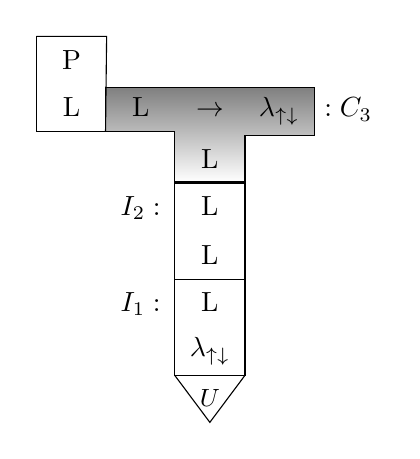
\begin{tikzpicture}
            \matrix (m) [matrix of nodes,nodes={minimum width=2.5em,minimum  height=1.7em}
                        ]
            {
              P     &            &                      &           &           \\
              L     &   L        & $\to$                & \mslang{} &  $:C_3$   \\
                    &            & L                    &           &           \\
                    &   $I_2:$   & L                    &           &           \\
                    &            & L                    &           &           \\
                    &   $I_1:$   & L                    &           &           \\
                    &            & \mslang{}            &           &           \\
                    &            & |[font=\small]|$U$   &           &           \\
             };
            \draw (m-1-1.north west) |- (m-2-1.south east);
            \draw (m-1-1.north west) -- (m-1-1.north east) -- (m-2-2.south west);
            \draw (m-2-2.south west) |- (m-2-4.north east) |- (m-2-3.south east) |- (m-4-3.north west) |- (m-2-2.south west);
            \draw (m-4-3.north west) |- (m-7-3.south east) |- (m-4-3.north west);
            \draw (m-3-3.south west) |- (m-3-3.south east);
            \draw (m-5-3.south west) |- (m-5-3.south east);
            \draw (m-7-3.south west) -- (m-8-3.south) -- (m-7-3.south east);

            % Background
            \begin{scope}[on background layer]
                \draw[shade] (m-2-2.south west) |- (m-2-4.north east) |- (m-2-3.south east) |- (m-4-3.north west) |- (m-2-2.south west);
            \end{scope}
    \end{tikzpicture}
    \caption{Tower whose top interpreter is staged (i.e., converted into a compiler, $C$)}
    \label{fig:tombstone_collapse_ex_comp}
    \end{subfigure}
    \begin{subfigure}{\linewidth}
    \centering
    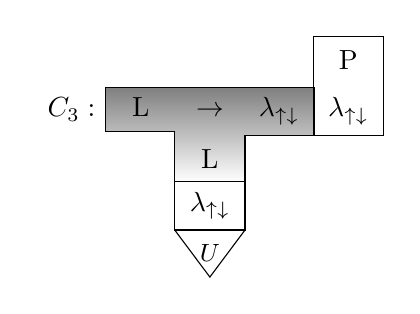
\begin{tikzpicture}
            \matrix (m) [matrix of nodes,nodes={minimum width=2.5em,minimum  height=1.7em}
                        ]
            {
        &     &                       &           &   P       \\
 $C_3:$ & L   & $\to$                 & \mslang   & \mslang   \\
        &     & L                     &           &           \\
        &     & \mslang{}             &           &           \\
        &     & |[font=\small]|$U$    &           &           \\
             };

            \draw (m-1-5.south west) |- (m-1-5.north east) |- (m-2-5.south east) -- (m-2-5.south west) -- (m-1-5.south west);
            \draw (m-2-2.south west) |- (m-2-4.north east) |- (m-2-3.south east) |- (m-4-3.north west) |- (m-2-2.south west);
            \draw (m-4-3.north west) |- (m-4-3.south east) |- (m-4-3.north west);
            \draw (m-4-3.south west) -- (m-5-3.south) -- (m-4-3.south east);

            % Background
            \begin{scope}[on background layer]
                \draw[shade] (m-2-2.south west) |- (m-2-4.north east) |- (m-2-3.south east) |- (m-4-3.north west) |- (m-2-2.south west);
            \end{scope}
    \end{tikzpicture}
    \caption{Final representation of the tower in \ref{fig:tombstone_collapse_ex_int} after collapsing it. All intermediate interpretation (levels $I_1$ to $I_3$) has been eliminated (by evaluating it during PE time) and $P$ has been specialized with respect to the top-most staged interpreter, $C_3$. The residual program $P$ consists of \mslang{} terms in ANF-normal form.}
    \label{fig:tombstone_collapsed}
    \end{subfigure}
    \caption{Tombstone diagrams representing the process of collapsing a tower using \mslang{}}
\end{figure}

Figures \ref{fig:tombstone_collapse_ex_int} to \ref{fig:tombstone_collapsed} depict the process of collapsing a (homogeneous) tower through tombstone diagrams. We start with a meta-circular tower of interpreters all written in the same language, $L$, and Pink's \mslang{} at the base. The key benefit of meta-circularity is that the \textit{lift} operator defined in \mslang{} is accessible to each interpreter. We can now stage some interpreter in the tower, in this example the user-most one, $I_3$, by lifting; this interpreter is now equivalent to a compiler from $L$ to \mslang{} ($C_3$ in figure \ref{fig:tombstone_collapse_ex_comp}). When we execute the tower (i.e., invoke \mslang's partial evaluator) $C_3$ residualizes while all other levels in the tower evaluate (essentially \textit{propagating} binding-time information of program $P$ from the top to the base of the tower). At $I_1$ a call to \textit{lift} now invokes \mslang's \textit{lift}. Effectively after residualization the generated program will only include the values staged at the top-most interpreter while the rest of the tower was reduced at specialization time. The result is a collapsed tower in figure \ref{fig:tombstone_collapsed} where all intermediate interpreters, $I_1$ through $I_3$, have been removed from the tower (assuming the absence of side-effects at individual levels).

\section{Heterogeneous Towers}\label{sec:heterogeneity}
A central part of our study revolves around the notion of heterogeneous towers. We continue from where Amin et al.'s study of collapsing towers of interpreters~\cite{amin2017collapsing} left off, namely the question of how one might achieve the effect of compiling multiple interpreters in heterogeneous settings. We view heterogeneous towers as a generalization of reflective towers and define \textit{heterogeneous} as follows:

\theoremstyle{definition}
\begin{definition}
	Heterogeneous towers of interpreters are systems of interpreters, $I^L_1, I^L_2, ..., I^L_n$ where $n,k \in \mathbb N_{\ge 1}$ and $I^L_k$ determines an interpreter at level $k$ written in language $L_{k-1}$ and interprets programs in $L_k$.
\end{definition}

%A level here is analogous to an instance of an interpreter within the tower and as such level $n$ implies $I_n$ if not mentioned explicitly otherwise.
\begin{observation}
    \label{def:het}
	Heterogeneous towers of interpreters are towers which generalize homogeneous towers by:
	\begin{enumerate}
		\item For any two adjacent interpreters $I_k$ and $I_{k-1}$ where $k \in \mathbb N_{\ge 1}: L_k \not\equiv L_{k-1}$ can hold
		\item For any two adjacent interpreters used in the tower, $I_{k}$ and $I_{k-1}$, the operational semantics and the representation of data can be different between the two even if the languages coincide; this gives us a way of addressing the difference in intensional structure between towers
	\end{enumerate}
\end{observation}

\subsection{Absence of: Meta-circularity}
The first generalization described by observation \ref{def:het} is that of mixed languages between levels of a tower. A practical challenge this poses for partial evaluators is the inability to reuse language facilities across interpreters. This also implies that one cannot in general define reflection and reification procedures as in 3-LISP~\cite{smith1984reflection}, Brown~\cite{wand1988mystery}, Blond~\cite{danvy1988intensions}, Black~\cite{asai1996duplication} or Pink~\cite{amin2017collapsing}.

\subsection{Absence of: Reflection}
Reflection in an interpreter enables the introspection and modification of its state during execution. It is a tool reflective languages can use to embed, for example, debuggers or run-time instrumentation into programs. Reflection in reflective towers implies the ability to modify an interpreter's interpreter which can be beneficial in the implementation of said tools. However, it also allows potentially destructive operations on a running interpreter's semantics which can become difficult to reason about or debug. Towers that we are interested in rarely provide reflective capabilities in their interpreters. Thus, we do not support or experiment with reflection in our study.

\begin{figure*}
    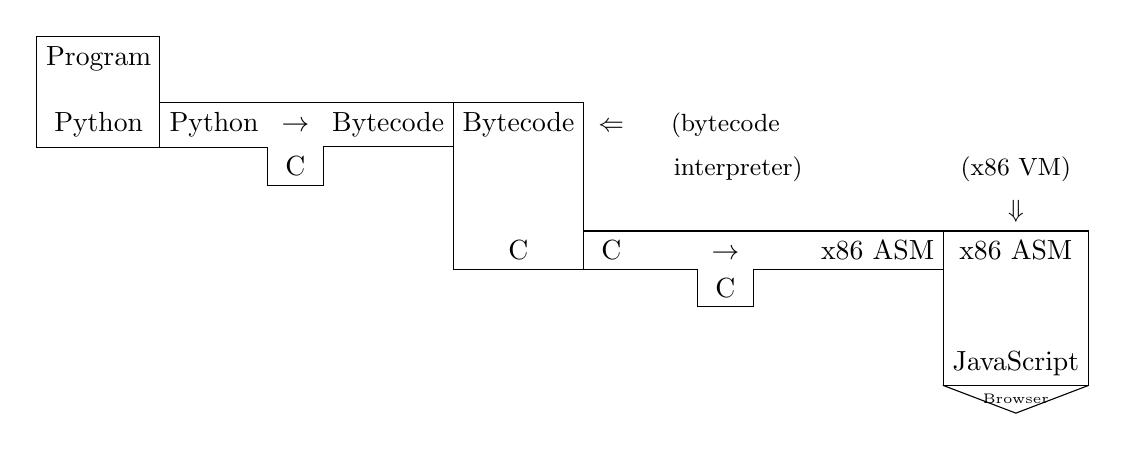
\begin{tikzpicture}
        \matrix (m) [matrix of nodes,nodes={minimum width=2em}
                    ]
        {
         Program    &        &        &           &           &     &       &           &               \\[2ex]
         Python     & Python &  $\to$ &  Bytecode &  Bytecode &   |[font=\small]|$\Leftarrow$  &  |[font=\small]|(bytecode  &           &               \\
                    &        &    C    &           &       &  & |[font=\small]|\quad interpreter) &           &   |[font=\small]|(x86 VM)         \\
                    &        &        &           &           &     &       &           &  |[font=\small]|$\Downarrow$         \\
                    &        &        &           &     C     &   C & $\to$ & x86 ASM   &  x86 ASM      \\
                    &        &        &           &           &     &   C   &           &               \\[3ex]
                    &        &        &           &           &     &       &           &  JavaScript   \\
                    &        &        &           &           &     &       &           &  |[font=\tiny]|Browser      \\
          };

        % Without arc
        \draw (m-1-1.north west) |- (m-2-2.south west) |- (m-1-1.north west);
        
        \draw (m-2-2.south west) |- (m-2-4.north east) |- (m-3-3.north east) |- (m-3-3.south west) |- (m-2-2.south west);
        \draw (m-2-4.north east) |- (m-5-7.south west) |- (m-6-7.south east) |- (m-5-8.south east) |- (m-7-9.south east) |- (m-5-6.north west) |- (m-2-4.north east);
        \draw (m-5-6.north west) -- (m-5-6.south west);
        \draw (m-5-8.north east) -- (m-5-8.south east);
        \draw (m-7-9.south west) -- (m-8-9.south) -- (m-7-9.south east);
    \end{tikzpicture}
    \caption{A hypothetical tower of interpreters that serves as the model for the tower we built (figure~\ref{fig:tombstone}). The diagram depicts a x86 virtual machine (VM) written in JavaScript running a Python~\cite{van2011python} interpreter that in turn executes some Python program. In this model, Python is first translated to bytecode which is then interpreted by some bytecode interpreter (written in the C language~\cite{kernighan1988c}). \textit{Browser} encompasses the JavaScript interpreter within a browser and any underlying technologies required to host the browser.}
    \label{fig:tombstone_practical}
\end{figure*}

\begin{figure*}
    \centering
        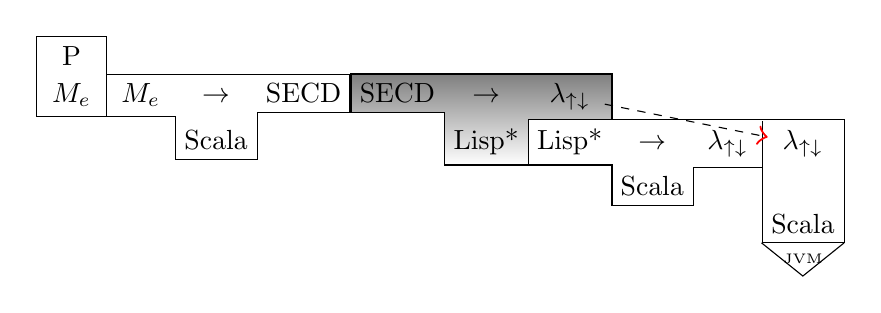
\begin{tikzpicture}
            \matrix (m) [matrix of nodes,nodes={minimum width=2.5em,minimum  height=1.2em}
                        ]
            {
        P       &       &       &       &       &       &         &         &         &                     \\
        \mevl   & \mevl & $\to$ & SECD  & SECD  & $\to$ & \mslang &         &         &                     \\
                &       & Scala &       &       & Lisp* &  Lisp*  & $\to$   & \mslang & \mslang             \\
                &       &       &       &       &       &         & Scala   &         &                     \\
                &       &       &       &       &       &         &         &         & Scala               \\
                &       &       &       &       &       &         &         &         & |[font=\tiny]|JVM \\
            };
            % Outline
            \draw (m-1-1.north west) |- (m-2-2.south east) |- (m-3-3.south east) |- (m-2-5.south east) |- (m-3-7.south east) |- (m-4-8.south east) |- (m-3-9.south east) |- (m-5-10.south east) |- (m-3-7.north east) |- (m-1-1.south east) |- (m-1-1.north west);

            % Dashes
            \draw (m-2-1.north east) -- (m-2-1.south east);
            \draw (m-2-4.north east) -- (m-2-4.south east);
            \draw (m-3-6.south east) |- (m-3-7.north east);
            \draw (m-3-9.north east) -- (m-3-9.south east);

            % Triangle
            \draw (m-5-10.south east) -- (m-6-10.south) -- (m-5-10.south west);

            % Background
            \begin{scope}[on background layer]
                \draw[shade] (m-2-5.north west) |- (m-2-5.south east) |- (m-3-6.south east) |- (m-3-7.north east) |- (m-2-5.north west);
            \end{scope}

            % Arrow
            \draw [big arrow] (m-2-7) -- (m-3-10);
        \end{tikzpicture}
    \caption{Our heterogeneous tower of interpreters (\ref{fig:tombstone}) after staging at the SECD level (shaded tombstone). All computation to the left of the staged interpreter is carried into the residual program. The collapse essentially moved the code from above the SECD machine to the base.}
    \label{fig:tombstone_het_collapse_secd}
\end{figure*}

\begin{figure*}
    \centering
        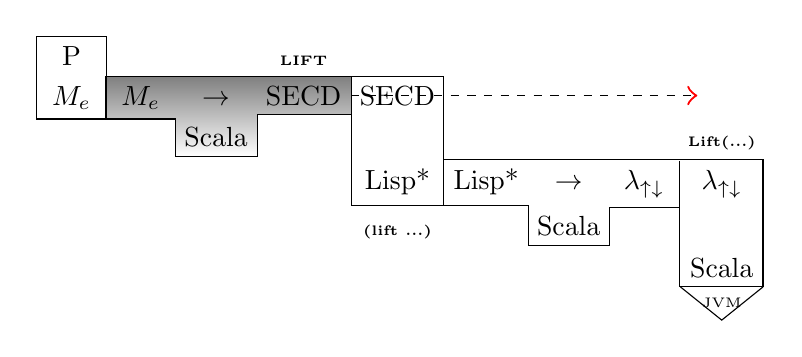
\begin{tikzpicture}
            \matrix (m) [matrix of nodes,nodes={minimum width=2.5em,minimum  height=1.2em}
                        ]
            {
P       &       &       & |[font=\tiny]|\textbf{LIFT}   &                                   &       &         &         &                                   \\
\mevl   & \mevl & $\to$ & SECD                          & SECD                              &       &         &         &                                   \\
        &       & Scala &                               &                                   &       &         &         & |[font=\tiny]|\textbf{Lift(...)}  \\
        &       &       &                               & Lisp*                             & Lisp* & $\to$   & \mslang & \mslang                           \\
        &       &       &                               & |[font=\tiny]|\textbf{(lift ...)}  &       & Scala   &         &                                   \\
        &       &       &                               &                                   &       &         &         & Scala                             \\
        &       &       &                               &                                   &       &         &         & |[font=\tiny]|JVM               \\
            };
            % Outline
            \draw (m-1-1.north west) |- (m-2-2.south east) |- (m-3-3.south east) |- (m-2-4.south east) |- (m-4-6.south east) |- (m-5-7.south east) |- (m-4-8.south east) |- (m-6-9.south east) |- (m-4-6.north west) |- (m-2-1.north east) |- (m-1-1.north west);

            % Dashes
            \draw (m-2-1.north east) -- (m-2-1.south east);
            \draw (m-2-4.north east) -- (m-2-4.south east);
            \draw (m-4-6.north west) |- (m-4-6.south west);
            \draw (m-4-8.north east) -- (m-4-8.south east);

            % Triangle
            \draw (m-6-9.south east) -- (m-7-9.south) -- (m-6-9.south west);

            % Background
            \begin{scope}[on background layer]
                \draw[shade] (m-2-2.north west) |- (m-2-2.south east) |- (m-3-3.south east) |- (m-2-4.south east) |- (m-2-2.north west);
            \end{scope}

            % Arrow
            \draw [big arrow] (m-2-4) --++(0:5cm);
        \end{tikzpicture}
    \caption{Our heterogeneous tower of interpreters after staging at the \mevl{} level (shaded tombstone). At each level, starting from \mevl, the \textit{lift} operator is implemented differently but together they achieve the effect of moving code from the \mevl{} interpreter to the base.}
    \label{fig:tombstone_het_collapse_mevl}
\end{figure*}

\subsection{Semantic Gaps}
Danvy et al.~mentioned the possibility of non-reflective non-meta-circular towers early on in his denotational description of the reflective tower model~\cite{danvy1988intensions}. The authors explored the idea of having different denotations for data at every level of the tower. However, since it was not the focus of their study, the potential consequences were not further investigated but serve as an inspiration for the second point of observation~\ref{def:het}. We call the difference in operational semantics or data representation between two interpreters a \textit{semantic gap}.

Another motivation of ours stems from the realization that systems consisting of several layers of interpretation can feasibly be constructed. A hypothetical tower of interpreters that served as a model for the one we built throughout our work was described in Amin et al.'s paper on collapsing towers~\cite{amin2017collapsing} and is depicted as a tombstone diagram in figure~\ref{fig:tombstone_practical}. As a comparison our tower is shown in figure~\ref{fig:tombstone}. We replace the x86 emulator with a SECD abstract machine interpreter and Python with our own functional toy language, \mevl. The label \mslang{} represents the multi-level core language from Pink~\cite{amin2017collapsing} and Lisp* is the Lisp-like front-end to \mslang. Although here the tower grows upwards and to the left, this need not be. We implement (in Scala) the compilers, or \textit{translators}, from \mevl{} to SECD and from Lisp* to \mslang{} purely for simplicity. To realize a completely vertical tower (i.e., consisting of interpreters only), the Lisp*--\mslang{} translator could be omitted so that the \mslang{} interpreter evaluates S-expressions directly. Similarly, the \mevl--SECD compiler could be implemented in SECD instructions itself. However, we argue that the presence of compilation layers in our experimental tower more closely resembles practice and adds some insightful challenges to our experiments.

%% We chose the SECD machine to create semantic gaps within our tower through the low-level instruction set that it comes with \cite{kogge1990architecture}. For convenience we chose to implement the \mevl{} level as a translator from \mevl{} to SECD instructions instead of writing the interpreter in the instructions directly.
%% It is noteworthy that the addition of translation layers to the tower revealed insights into the process of collapsing heterogeneous towers that are not immediately apparent from the composition of tombstones, as we see next. \todo{this paragraph is kind of a repition of the last sentence of the one above; perhaps merge the two paragraphs}


\section{Collapsing Heterogeneous Towers}\label{subsec:collapseh}
We describe our observations and further effects of heterogeneity on collapsing towers.
First, as an echo to section~\ref{subsec:collapse} and as a summary, the key ingredients for collapsing a heterogeneous tower are:
\begin{enumerate}
    \item A multi-level base language
    \item A \textit{lift} operator
    \item A staged user-most evaluator
    \item Unstaged lower evaluators
    \item \textbf{New requirement: } The \textit{lift} operator must be exposed in each evaluator, and must translate from that level's values to the lower-level values.
\end{enumerate}

We can stage the SECD machine, even though doing so is unlikely to be
optimal as it is not the user-most interpreter.
While a definitional interpreter can be staged using TDPE by simply lifting
its return values, the process of staging an abstract machine requires a more sophisticated binding-time analysis with careful ({\it i\/}) design of its division rules
and ({\it ii\/}) decision on which expressions 
to lift to avoid non-termination at PE-time.
Figure~\ref{fig:tombstone_het_collapse_secd} depicts the effect of staging the SECD interpreter in our tower. After staging the SECD machine (highlighted in grey) it now operates as a compiler from SECD instructions to \mslang{} terms. Collapsing the tower in this configuration essentially means moving code from the SECD level to the base interpreter across the Lisp* level. Consistent with the composition rules of tombstones, the levels above SECD are residualized and present in the output as well.

To stage the \mevl{} evaluator, above the SECD machine, requires a \textit{lift} operator. There are two difficulties.
%%AM: moved back to enumerate given we have space!
\begin{enumerate}
\item
In mixed-language towers a \textit{lift} operation is not available to an interpreter unless explicitly provided at each given level.
Hence, one approach to propagating binding-time information is to implement a built-in \textit{lift} at all levels below the interpreter that is to be staged. The implementation of \textit{lift} may require us to reverse engineer and transform the representation of closures, pairs or other constructs which the \textit{lift} at the base expects.

\item
A more subtle collapse of our tower occurs when we stage the \mevl{} level (see figure \ref{fig:tombstone_het_collapse_mevl}). In this case staging has a slightly different effect which is not obvious from the tombstones. Since the \mevl{} level is actually a translator already, staging the translator will simply yield another translator. Instead, staging \mevl{} means we generate SECD code that \textit{lifts} (i.e., signals the PE to residualize) expressions of \mevl{} using a new \textbf{LIFT} instruction. As we can see from the annotated tombstone diagram, we use the \textit{lift} operator as a mechanism to move code through each level to the base where it is residualized.
\end{enumerate}

The \textbf{LIFT} instruction in the SECD machine has to create
closures understood by the lower level. In order to do so, it must
reverse engineer the representation of closures, which, for recursive
functions, can be implicit in the wiring of the SECD machine. These changes cross-cut the original design, adding complexity.
For example, adding support for the \textbf{LIFT} instruction to an otherwise standard SECD machine interpreter
requires adapting the following instructions:
\begin{description}
\item [LDF] which loads instructions as a function, now requires tagging, so that closure values can be distinguished from others
\item [AP ] which applies a function, now requires deciding whether to apply or generate code for application (to avoid infinite unrolling)
\item [RTN] which returns from a function, now requires deciding whether to restore state of registers with the dump (default) or return a value to satisfy calling convention of the interpreters below the SECD machine
\end{description}

This study demonstrates that it is feasible to collapse a particular
heterogeneous tower. The SECD machine acts as a bottleneck
between two Lisp-like levels, because it forces a different lower
stack-based representation. Collapsing the tower removes
all interpretive overhead, translating from one Lisp to the other,
without suffering any obfuscation due to the SECD machine.

The general lesson for collapsing towers is that each level must be
able to lift values by translating them to the lower level. In
practice, this presents various difficulties.

\section{Conclusions and Future Work}\label{sec:conc}

%AM:\subsection{Conclusions}
%% The aim of our study was to connect the extensive collection of work on homogeneous reflective towers with their counterparts in more practical settings. Collapsing of towers of interpreters encompasses the techniques to remove interpretative overhead that is present in such systems. The construction of towers of interpreters has previously been either limited to reflective towers, in which each interpreter is meta-circular and exposes its internals for the purpose of reflection, or a consequence of modular systems design where layers of tools that perform some form of interpretation are glued together. To the best of our knowledge, our work is one of a handful, together with Amin et al.'s previous explorations~\cite{amin2017collapsing}, that explicitly focus on the overheads and optimization of towers of interpreters that are not meta-circular. We built on the ideas from the Pink framework and re-used its TDPE-based partial evaluator to construct and collapse our own experimental tower.

%% A tower of meta-circular interpreters can be collapsed into a residual program in a single pass by only staging a single interpreter in the tower and relying on the meta-circular definitions of \textit{lift} to propagate binding-time information to the multi-level base evaluator which handles the actual code generation (in Pink through an embedded partial evaluator).
We started by generalizing the concept of reflective towers to ones that consisted of non-meta-circular interpreters. To model a tower that could potentially contain layers of translation between languages, such as the one in figure \ref{fig:tombstone_practical}, we also introduced the notion of \textit{semantic gaps}, which dictate the extent to which two adjacent interpreters differ in operational semantics or representation of data. A combination of these two properties (non-meta-circularity and semantic gaps) form the new class of towers of interpreters that we call \textit{heterogeneous}. The theoretical implications from heterogeneity on a tower's structure and procedure to collapse them was a focal point for our experiments. We envisioned two problems with collapsing heterogeneous towers:
\begin{enumerate*}[label=(\arabic*)]
    \item we needed to devise a strategy to signal to the PE at the base of the tower which expressions to residualize without a meta-circular \textit{lift} (even through levels of compilation)
    \item semantic gaps required us to perform complex transformations on program constructs in one interpreter to adhere to their representation in adjacent interpreters
\end{enumerate*}. We constructed and then collapsed a 5-level heterogeneous tower with a SECD machine as one of its levels to provide evidence for these hypotheses and gain more insights into heterogeneity.

Staging an interpreter amounts to reifying literals, lambdas and product types it returns. An abstract machine is not guaranteed to distinguish these types by data structures or a type-system but can instead rely on dedicated instructions to differentiate data of these types. Hence, the points to reify at are dictated by the architecture of the underlying machine. In our experiments we created a conservative division (of variables into static and dynamic)
tailored to the SECD registers
and reduced static expressions in Pink's reflect operator to achieve optimal residualization. In order to propagate the decision of whether to generate or evaluate an expression through levels in the tower, we implemented a \textit{lift} operation for all languages in the tower. Observationally, \textit{lifting} an expression moves it through the tower to the base and is the key to achieving the effect of collapsing. Whereas in homogeneous towers this role of \textit{lift} was implicit and trivial due to meta-circularity, we found that heterogeneity explicates this process. We hope this furthered the understanding of some of the subtleties of collapsing towers of interpreters.

The type of overhead our study concerned itself with was the dispatch logic in an interpreter that decides which operation to perform based on the current term being evaluated. The interpretative cost we removed in a tower is that between the base evaluator and the top-most staged level. We used our experimental tower to investigate the effect of staging interpreters at various points. As expected, the interpretative overhead of all levels up to the one being staged was completely reduced during specialization time. More notably, the structure of the generated code followed that of the interpreter that was staged. In our case, staging at the SECD machine level generated code that contained traces of the SECD semantics such as stack-based operations and as a result still optimizable to the programmer. In comparison, staging at a level above yielded a residual program without any signs of SECD and more optimal for our example programs.

With our experiments we demonstrated the successful collapse of a heterogeneous tower. We also showed the ability of a TDPE-style \textit{reify} operation to essentially move code across levels of a tower, which also worked across levels of compilation. However, realizing our methodology on a practical setting such as the Python--x86--JavaScript tower will require additional work. Our approach to propagating the TDPE binding-time information involved the implementation of a reification operator in each interpreter that is missing it. This then required the reverse-engineering and conversion of types in an interpreter to the representation that the interpreter below in the tower expects. In practice these changes would require intimate knowledge of and intrusive changes to an interpreter or compiler. Additionally, in our experimental tower we did not consider the residualization of side-effects which a useful collapse procedure would need for wider applicability. Our methodology could, however, help the optimization of smaller-scale systems in practice where towers consist of embedded DSL interpreters or regular expression matchers (even in the absence of meta-circularity and presence of translation layers).

\paragraph{Future Work}

We hope our study provided a platform and the necessary techniques to eventually make collapsing towers in practice a reality. The next step is to extend our definition of heterogeneity to investigate ways of dealing with side-effects at various levels of a tower. The ability to perform side-effects such as destructive data structure changes are essential in real-world programs regardless of their domain but were not considered in our study.

One of the considerations is whether side-effects should be residualized, removed or executed during PE time. More broadly a next step would be to devise a method of dealing with situations where a level does not have a necessary feature that an interpreter in a different level requires.
Currently any feature, including side-effects, needs to be implemented at each level from the base up to the interpreter that uses it.
Kogge presents various extensions to the SECD machine such as a call/cc operator, lazy evaluation or even concurrency (through MultiLisp)~\cite{kogge1990architecture}. Implementing such extensions could aid the experimentation with features not being available at adjacent levels. For example, call/cc allows us to emulate side-effects such as such as exceptions and non-determinism.

%Nothing restricts our heterogeneous tower to using a SECD abstract machine. Instead further work could experiment with others like the Warren Abstract Machine (WAM)~\cite{warren1983abstract} as a SECD replacement. This would allow us to investigate the applicability of our method for collapsing towers to other programming paradigms such as logic programming. Even in the presence of the SECD machine we could replace the interpreters running on it, in our case \mevl, with higher-level logic-programming interpreters instead of the lower-level WAM. This could lead into a study of stratifications of towers and the extent to which certain types of towers are collapsible.

%A major subject of focus in PE is the ability to output residual programs in a language different from the subject language or the one the PE was written in. This could prove useful when staging between a fixed set of levels that is not the whole tower. Such a feature would need to be supported by the underlying PE methodology (i.e., TDPE in our case).

Ongoing work involves generalizing and making our technique to collapse towers less intrusive. Instead of reimplementing a \textit{lift} operation at the levels that need it, feasible techniques could, at least for particular domains or languages, pass the TDPE binding-time information in the form of data through each level. W{\"u}rthinger's GraalVM~\cite{wurthinger2013one} allows the communication between languages that target the Graal Virtual Machine and could prove useful in further experimenting with heterogeneous towers where multiple interpreters pass, e.g., binding-times to each other.

%%
%% The acknowledgments section is defined using the "acks" environment
%% (and NOT an unnumbered section). This ensures the proper
%% identification of the section in the article metadata, and the
%% consistent spelling of the heading.
\begin{acks}
\textit{placeholder}
\end{acks}

%%
%% The next two lines define the bibliography style to be used, and
%% the bibliography file.
\bibliographystyle{ACM-Reference-Format}
\bibliography{gpce}

%%
%% If your work has an appendix, this is the place to put it.
%\appendix

\end{document}
\endinput
%%
%% End of file `sample-sigplan.tex'.